\documentclass[conference]{IEEEtran}
\IEEEoverridecommandlockouts
\usepackage{cite}
\usepackage{amsmath,amssymb,amsfonts}
\usepackage{graphicx}
\usepackage{textcomp}
\usepackage{xcolor}
\usepackage{booktabs}
\usepackage{multirow}
\usepackage{array}
\usepackage{url}
\def\BibTeX{{\rm B\kern-.05em{\sc i\kern-.025em b}\kern-.08em
    T\kern-.1667em\lower.7ex\hbox{E}\kern-.125emX}}
\newcommand{\yes}{\checkmark}
\newcommand{\no}{--}

\begin{document}

\title{HEAL-GTN: Mining Longitudinal Electronic Health Records with a Hierarchical Graph-Temporal Network for Early Sepsis, Acute Kidney Injury and Mortality Prediction}

\author{\IEEEauthorblockN{Sathishkumar Veerappampalayam Easwaramoorthy}
\IEEEauthorblockA{\textit{Faculty of Engineering and Technology} \\
\textit{Sunway University}\\
Bandar Sunway, Selangor 47500, Malaysia \\
srisathishkumarve@gmail.com}
\and
\IEEEauthorblockN{Abraheem Rashid}
\IEEEauthorblockA{\textit{Department of Computer Science} \\
\textit{Brunel University London}\\
Uxbridge UB8 3PH, United Kingdom \\
2546393@brunel.ac.uk}
}

\maketitle

\begin{abstract}
Risk prediction for sepsis, acute kidney injury and in-hospital death requires combining clinical notes, physiological measurements and coded diagnoses from electronic health records. Existing models usually encode these sources separately or as flat sequences, so they ignore the typed relations between clinical concepts and seldom report calibration or privacy settings. This study asks whether modeling those relations, together with learned fusion of the data sources, improves discrimination and calibration over strong sequence and language-model baselines. The question matters because poorly calibrated alerts cause alarm fatigue, and multi-site training is often restricted by privacy rules. We propose HEAL-GTN, a hierarchical graph-temporal network. It encodes notes with Clinical-BERT, vital signs with a multi-scale convolutional network and laboratory values with a multilayer perceptron, fuses them by cross-modal attention, propagates the fused patient vector through three heterogeneous graph-attention layers over diagnosis, medication and observation concepts, and summarizes time with a bidirectional LSTM and self-attention. Training combines focal and Cox losses with isotonic recalibration, and a federated variant applies differentially private gradient descent at 10 simulated sites. On 65,366 MIMIC-IV intensive care stays, HEAL-GTN reaches an AUROC of 0.912 for sepsis, 0.889 for acute kidney injury and 0.905 for mortality, which is 3.4, 4.0 and 2.9 points above the strongest of 17 baselines, and it lowers the expected calibration error for acute kidney injury from 0.062 to 0.028. Inference takes 27 ms per patient on a CPU. Because the outcomes are admission-level labels, these results describe retrospective risk stratification rather than prospective early warning.
\end{abstract}

\begin{IEEEkeywords}
Clinical data mining, electronic health records, heterogeneous graph attention, sepsis, acute kidney injury, calibration, federated learning, differential privacy.
\end{IEEEkeywords}

\section{Introduction}
Mining the notes, measurements, orders and codes that hospitals record for every admission is a long-standing goal of clinical informatics \cite{jensen2012,miotto2018}. Three outcomes in intensive care receive particular attention: sepsis, defined by the Sepsis-3 consensus \cite{singer2016}; acute kidney injury (AKI), staged by the KDIGO guideline \cite{kdigo2012}; and in-hospital mortality, a standard benchmark task on public critical care data \cite{johnson2017mlhc}. Deployed sepsis models have performed worse in external validation than during development \cite{wong2021}, and their accuracy falls further when only predictions made before clinicians begin treatment are counted \cite{kamran2024}. These findings make calibration, the timing of model inputs and transparent reporting central requirements rather than secondary details.

Electronic health record (EHR) data pose three difficulties. An intensive care unit (ICU) stay mixes dense vital-sign series, irregular laboratory panels, free-text notes and codes; the concepts are related, since diseases co-occur and drugs are prescribed for diagnoses; and the outcomes are rare, with 4.7\% of stays in our MIMIC-IV cohort labeled sepsis and 6.8\% AKI.

Recurrent and attention models handle measurement sequences \cite{harutyunyan2019,ma2017dipole,song2018sand}, transformers model ordered code sequences \cite{li2020behrt,rasmy2021medbert,li2023hibehrt,yang2023transformehr}, and pretrained language models encode clinical text \cite{alsentzer2019,yang2022gatortron,jiang2023nyutron}. Graph methods add ontology and co-occurrence structure \cite{choi2017gram,choi2020gct,jiang2024graphcare}. Four gaps remain. Most models treat the record as a flat sequence and do not use typed relations between concepts. Modalities are usually combined by concatenation rather than learned attention, although recent work shows the value of learned multimodal fusion \cite{zhang2023icml}. Calibration is rarely reported, even though it determines whether risk scores can be thresholded safely \cite{vancalster2019}. Finally, privacy settings for multi-site training are seldom given in a form that allows the privacy budget to be recomputed \cite{ponomareva2023}.

This paper presents HEAL-GTN, a hierarchical graph-temporal network that addresses these gaps. Its contributions are as follows.
\begin{enumerate}
\item A per-stay heterogeneous patient-concept graph with five node types and six typed relations, processed by relation-specific GATv2 attention with learnable relation weights.
\item A hierarchical architecture that encodes notes, vital signs, laboratory values and codes separately, fuses them with cross-modal attention, propagates the fused patient vector through the graph, and summarizes time with a bidirectional LSTM and self-attention. Training combines focal loss, a Cox partial likelihood and a counterfactual consistency penalty, followed by isotonic recalibration.
\item A federated training protocol with differentially private stochastic gradient descent, reported with every setting needed to recompute its per-round privacy budget.
\item A comparison with 17 baselines on MIMIC-IV, with ablations, calibration, transfer to eICU-CRD, robustness and subgroup analyses, and an explicit account of which inputs are available at prediction time and where leakage could arise.
\end{enumerate}

\section{Related Work}
\subsection{Sequence and Transformer Models for EHR Data}
RETAIN introduced reverse-time attention over visits \cite{choi2016retain}, Dipole combined bidirectional recurrence with attention \cite{ma2017dipole}, and SAnD applied self-attention to clinical time series \cite{song2018sand}. Harutyunyan \textit{et al.} established LSTM benchmarks for mortality and other tasks on MIMIC-III \cite{harutyunyan2019}, and DeepSurv coupled neural networks with the Cox model \cite{katzman2018deepsurv}. BEHRT \cite{li2020behrt} and Med-BERT \cite{rasmy2021medbert} pretrain transformers on code sequences; Hi-BEHRT extends this to long multimodal histories with a hierarchical transformer \cite{li2023hibehrt}, and TransformEHR uses an encoder-decoder objective that predicts all outcomes of a future visit \cite{yang2023transformehr}. These models capture order but treat codes as tokens without typed relations.

\subsection{Clinical Language and Foundation Models}
Clinical-BERT \cite{alsentzer2019}, BioGPT \cite{luo2022biogpt}, GatorTron \cite{yang2022gatortron} and NYUTron \cite{jiang2023nyutron} encode clinical or biomedical text, and NYUTron showed that a language model trained on notes from one health system can predict readmission and mortality. A review of 84 EHR foundation models found that most are evaluated on narrow public datasets and on tasks with limited operational value \cite{wornow2023}. Zhang \textit{et al.} model irregular time series and notes jointly with interleaved attention \cite{zhang2023icml}. HEAL-GTN uses a clinical language model as one encoder within a graph-based model instead of relying on text alone.

\subsection{Graph Neural Networks in Healthcare}
GRAM injects the ICD hierarchy into code embeddings \cite{choi2017gram}, GCT learns the latent graph between codes in an encounter \cite{choi2020gct}, HeteroMed builds a heterogeneous information network for diagnosis \cite{hosseini2018heteromed}, and GraphCare builds personalized knowledge graphs with help from large language models \cite{jiang2024graphcare}. HEAL-GTN builds on graph attention \cite{brody2022} and on heterogeneous attention over typed relations \cite{wang2019han}, and it differs from the works above in using the graph as the point where modality-specific information is fused.

\subsection{Privacy-Preserving and Federated Clinical Learning}
Federated averaging \cite{mcmahan2017} and DP-SGD \cite{abadi2016} are the standard tools for multi-site training. Federated learning has been proposed as a route to multi-institution clinical models \cite{rieke2020}, and the EXAM study trained a COVID-19 outcome model across 20 institutions \cite{dayan2021}. Ponomareva \textit{et al.} give practical guidance on which DP settings to report so that a guarantee can be checked \cite{ponomareva2023}, and we follow it in Section~\ref{sec:dp}.

\subsection{Leakage and Evaluation Practice}
Leakage between training data and evaluation targets has inflated results in many fields that use machine learning \cite{kapoor2023}. In sepsis prediction, models can appear accurate because they react to signs of clinical suspicion that are themselves recorded after the clinicians have recognized the condition \cite{kamran2024}. Multi-site benchmarks such as YAIB \cite{vandewater2024} and the international validation by Moor \textit{et al.} \cite{moor2023} show how much reported performance depends on the cohort, the label definition and the site, MIMIC cohorts are hard to reproduce from published descriptions \cite{johnson2017mlhc}, and machine learning for health lags other fields in sharing data and code \cite{mcdermott2021}. Table~\ref{tab:position} places HEAL-GTN against representative systems. None of them covers all six properties.

\begin{table}[t]
\caption{Data sources and design properties of representative systems}
\label{tab:position}
\centering
\footnotesize
\setlength{\tabcolsep}{2.6pt}
\begin{tabular}{@{}lcccccc@{}}
\toprule
Method & Codes & Notes & Vitals/labs & Graph & Fusion & Federated \\
\midrule
RETAIN \cite{choi2016retain} & \yes & \no & \no & \no & \no & \no \\
LSTM \cite{harutyunyan2019} & \no & \no & \yes & \no & \no & \no \\
Clinical-BERT \cite{alsentzer2019} & \no & \yes & \no & \no & \no & \no \\
BEHRT \cite{li2020behrt} & \yes & \no & \no & \no & \no & \no \\
GRAM \cite{choi2017gram} & \yes & \no & \no & \yes & \no & \no \\
GraphCare \cite{jiang2024graphcare} & \yes & \no & \no & \yes & \no & \no \\
Zhang \textit{et al.} \cite{zhang2023icml} & \no & \yes & \yes & \no & \yes & \no \\
EXAM \cite{dayan2021} & \no & \no & \yes & \no & \yes & \yes \\
\midrule
HEAL-GTN (ours) & \yes & \yes & \yes & \yes & \yes & \yes \\
\bottomrule
\end{tabular}
\end{table}

\section{Problem Formulation}\label{sec:problem}
\textit{Data.} Let $\mathcal{D}=\{(\mathcal{E}_i,\mathbf{y}_i)\}_{i=1}^{N}$ be a cohort of ICU stays. Stay $i$ is an event stream $\mathcal{E}_i=\{(x_{ij},m_{ij},\tau_{ij})\}_j$, where $x_{ij}$ is a value, $m_{ij}\in\mathcal{M}$ its modality and $\tau_{ij}$ the time at which it became available in the record. The modalities are $\mathcal{M}=\{\text{note},\text{vital},\text{lab},\text{code}\}$. From $\mathcal{E}_i$ we derive a note set $X^{n}_i$, a vital-sign matrix $X^{v}_i\in\mathbb{R}^{T\times F_v}$ on an hourly grid of length $T$, a laboratory and demographic vector $\mathbf{x}^{\ell}_i\in\mathbb{R}^{F_\ell}$, and three code sets $C^{d}_i$, $C^{m}_i$ and $C^{o}_i$ for diagnoses, medications and observations.

\textit{Information set.} For a prediction time $t$, the information available about stay $i$ is
\begin{equation}
\mathcal{H}_i(t)=\{(x_{ij},m_{ij},\tau_{ij})\in\mathcal{E}_i:\tau_{ij}\le t\}.
\label{eq:info}
\end{equation}
A model is temporally admissible if its output at time $t$ depends only on $\mathcal{H}_i(t)$. Section~\ref{sec:availability} states which inputs of the reported experiments meet this condition.

\textit{Graph.} Each stay is represented by a heterogeneous graph $G_i=(V_i,E_i,\phi,\psi)$ with node-type map $\phi:V_i\rightarrow\mathcal{A}$ and edge-type map $\psi:E_i\rightarrow\mathcal{R}$, where $\mathcal{A}$ contains the five node types patient, diagnosis, medication, observation and encounter, and $\mathcal{R}$ contains the six relations has-diagnosis, prescribed, observed, during, follows and co-occurs.
Concept nodes are drawn from $C^{d}_i\cup C^{m}_i\cup C^{o}_i$, and there is one encounter node per hospital day. $G_i$ is built from stay $i$ alone, so no node in it belongs to another patient.

\textit{Outcomes.} Each stay has labels $\mathbf{y}_i=(y^{s}_i,y^{a}_i,T_i,\delta_i)$, where $y^{s}_i,y^{a}_i\in\{0,1\}$ indicate sepsis and AKI during the admission, $T_i$ is the time from admission to death or discharge, and $\delta_i=1$ if the patient died in hospital. Section~\ref{sec:data} gives the exact definitions.

\textit{Learning problem.} A model $f_\theta$ maps the inputs of stay $i$ to a shared representation $\mathbf{h}_i$ and three outputs: $\hat{y}^{s}_i=\sigma(g_s(\mathbf{h}_i))$, $\hat{y}^{a}_i=\sigma(g_a(\mathbf{h}_i))$ and a log-risk $r_i=g_m(\mathbf{h}_i)$ for the proportional hazards model. Training minimizes
\begin{equation}
\mathcal{L}(\theta)=\mathcal{L}_{\mathrm{foc}}^{s}+\mathcal{L}_{\mathrm{foc}}^{a}+\lambda_{\mathrm{cox}}\mathcal{L}_{\mathrm{cox}}+\lambda_{\mathrm{cf}}\mathcal{L}_{\mathrm{cf}},
\label{eq:objective}
\end{equation}
with the terms defined in Section~\ref{sec:loss}.

\textit{Federated constraint.} In the federated setting the training data are split into disjoint site datasets $\mathcal{D}=\bigcup_{k=1}^{K}\mathcal{D}_k$, and records never leave their site. A randomized mechanism $\mathcal{M}$ is $(\varepsilon,\delta)$-differentially private if, for any two datasets $D$ and $D'$ that differ in one record and any set of outputs $S$,
\begin{equation}
\Pr[\mathcal{M}(D)\in S]\le e^{\varepsilon}\Pr[\mathcal{M}(D')\in S]+\delta.
\label{eq:dp}
\end{equation}
We require each site's update in a communication round to satisfy (\ref{eq:dp}) with respect to that site's records.

\textit{Evaluation.} Discrimination is measured by the area under the ROC curve (AUROC) and calibration by the expected calibration error (ECE).

\section{Proposed HEAL-GTN Framework}
Fig.~\ref{fig:arch} shows the architecture and Fig.~\ref{fig:graph} the graph schema.

\begin{figure*}[t]
\centering
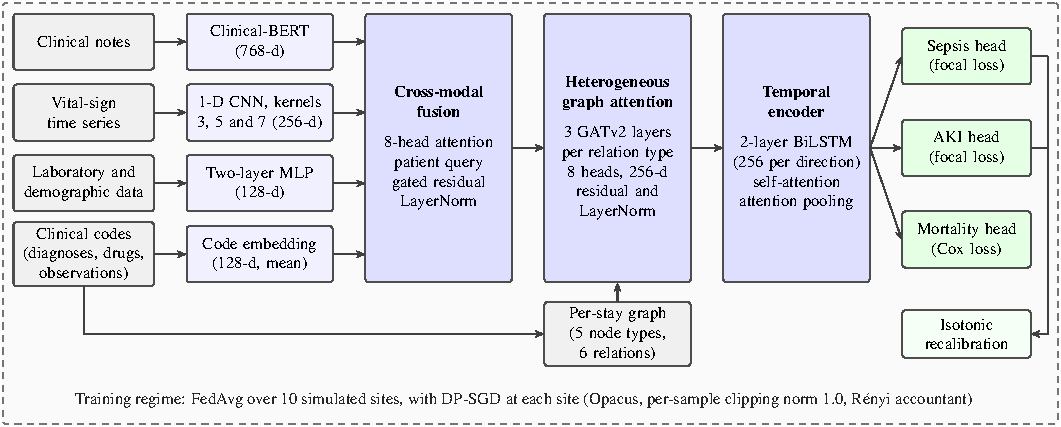
\includegraphics{figures/fig1_architecture.pdf}
\caption{HEAL-GTN architecture. Modality encoders feed a cross-modal fusion block whose output becomes the patient node of a per-stay heterogeneous graph. Three heterogeneous graph-attention layers and a temporal encoder produce the representation used by the sepsis, AKI and mortality heads. The dashed region marks the federated training regime.}
\label{fig:arch}
\end{figure*}

\subsection{Heterogeneous Patient-Concept Graph}
The graph of stay $i$ follows the schema in Fig.~\ref{fig:graph}. Diagnosis nodes are ICD-10 codes, medication nodes are RxNorm concepts and observation nodes are LOINC laboratory and vital-sign concepts. The patient node connects to every concept node of the stay through the has-diagnosis, prescribed and observed relations, and to one encounter node per hospital day through the during relation. Encounter nodes form a chain under the follows relation, and diagnoses recorded in the same stay are linked pairwise by co-occurs. Concept nodes are initialized from code embeddings, encounter nodes are initialized to zero, and the patient node receives the fused vector of Section~\ref{sec:fusion}. Because each graph contains only the codes of one stay, the graph structure carries no information from other patients, and all embeddings and relation weights are learned on the training split only.

\begin{figure}[t]
\centering
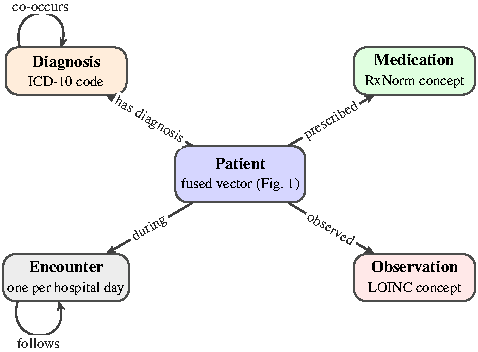
\includegraphics{figures/fig2_graph_schema.pdf}
\caption{Schema of the per-stay heterogeneous graph: five node types and six relation types. Arrows give the message direction used by the graph-attention layers.}
\label{fig:graph}
\end{figure}

\subsection{Modality Encoders and Cross-Modal Fusion}\label{sec:fusion}
Notes are encoded by Clinical-BERT \cite{alsentzer2019} with the lower eight transformer layers frozen, and the [CLS] vector (768-d) is used. Vital signs are encoded by a multi-scale one-dimensional CNN with three branches (kernel sizes 3, 5 and 7), each of two convolutions with 128 channels and global average pooling, followed by a projection to 256-d. Laboratory and demographic values pass through a two-layer MLP (128-d), and the code set is embedded (128-d) and mean-pooled. Each modality vector is projected to 256-d, and the four vectors form the key and value set $\mathbf{M}_i$ of an 8-head attention layer whose query $\mathbf{q}$ is a learned vector. With $\mathbf{a}_i=\mathrm{MHA}(\mathbf{q},\mathbf{M}_i,\mathbf{M}_i)$, the fused patient vector is
\begin{equation}
\mathbf{h}^{p}_i=\mathrm{LN}\big(\mathbf{q}+\sigma(\mathbf{W}_g[\mathbf{q}\,\|\,\mathbf{a}_i])\odot\mathbf{a}_i\big),
\label{eq:fusion}
\end{equation}
where $\sigma$ is the logistic function, $\|$ denotes concatenation and LN is layer normalization. Both the attention weights and the gate vary from stay to stay, so the model can rely less on a sparse modality, for example when few notes are available.

\subsection{Heterogeneous Graph-Attention Stack}
Three layers propagate information along typed edges. For relation $r$ with source node $s$ and destination node $d$, a GATv2 operator \cite{brody2022} computes
\begin{equation}
\alpha^{r}_{sd}=\operatorname{softmax}_{s\in\mathcal{N}_r(d)}\Big(\mathbf{a}_r^{\top}\,\mathrm{LeakyReLU}\big(\mathbf{W}_r[\mathbf{h}_s\,\|\,\mathbf{h}_d]\big)\Big),
\label{eq:gat}
\end{equation}
and the message $\mathbf{m}^{r}_d=\sum_{s}\alpha^{r}_{sd}\mathbf{W}'_r\mathbf{h}_s$, with eight heads concatenated to 256-d. Messages from different relations are combined with learnable scalar weights $\beta_r$, and each layer updates the node states as
\begin{equation}
\mathbf{h}^{(l+1)}_d=\mathbf{h}^{(l)}_d+\mathrm{LN}\Big(\mathrm{Drop}\big(\mathrm{GELU}\big(\textstyle\sum_{r}\beta_r\mathbf{m}^{r}_d\big)\big)\Big).
\label{eq:layer}
\end{equation}
Dropout of 0.1 on node states and on attention coefficients reduces over-fitting, and the residual connections limit over-smoothing as layers are added.

\subsection{Temporal Encoder}
The patient states of successive encounters form a sequence that a two-layer bidirectional LSTM with 256 units per direction processes. Its outputs are projected to 256-d and passed through multi-head self-attention with a residual connection and layer normalization, which links distant events such as a lactate rise and a later creatinine change. A second attention step with a learned query pools the sequence into the representation $\mathbf{h}_i$.

\subsection{Task Heads and Training Objective}\label{sec:loss}
Each head is a two-layer MLP with 128 hidden units. Sepsis and AKI use the focal loss \cite{lin2017focal}, $\ell=-\alpha_t(1-p_t)^{\gamma}\log p_t$ with $\gamma=2$ and $\alpha=0.25$, to reduce the weight of easy negatives. Mortality uses the negative Cox partial log-likelihood \cite{katzman2018deepsurv},
\begin{equation}
\mathcal{L}_{\mathrm{cox}}=-\frac{1}{\sum_i\delta_i}\sum_{i}\delta_i\Big(r_i-\log\sum_{j:T_j\ge T_i}e^{r_j}\Big),
\label{eq:cox}
\end{equation}
computed within each mini-batch. The counterfactual term $\mathcal{L}_{\mathrm{cf}}$ applies perturbations whose clinical direction is known, for example normalizing an abnormal lactate value, and adds a hinge penalty with margin 0.05 when the predicted risk moves in the wrong direction. The weights $\lambda_{\mathrm{cox}}=0.5$ and $\lambda_{\mathrm{cf}}=0.1$ in (\ref{eq:objective}) were selected by a 60-trial tree-structured Parzen estimator search \cite{bergstra2011} on the validation split. We train with AdamW (learning rate $3\times10^{-4}$, weight decay $10^{-5}$), a linear warm-up over 500 steps, gradient clipping at 1.0, batch size 32 and at most 60 epochs, and we keep the checkpoint with the lowest validation loss.

\subsection{Post-hoc Calibration}
Neural classifiers are often over-confident \cite{guo2017}. We fit an isotonic regression to the sepsis and AKI scores on the validation split and apply it unchanged to the test split. Isotonic regression is monotone, so it changes calibration but leaves the ranking of patients, and therefore the AUROC, almost unchanged.

\subsection{Differentially Private Federated Training}\label{sec:dp}
In the federated variant, $K=10$ sites train locally and a server combines their parameters by FedAvg \cite{mcmahan2017}, weighting each site by its number of training stays. All sites take part in each of 120 rounds, and each site runs two local epochs with batch size 16 and learning rate $10^{-4}$. Local training uses DP-SGD \cite{abadi2016} as implemented in Opacus \cite{yousefpour2021}: per-sample gradients are clipped to an $\ell_2$ norm of $C=1.0$, Gaussian noise is added, and the R\'enyi DP accountant \cite{mironov2017} calibrates the noise multiplier so that the two local epochs of one round satisfy $(\varepsilon,\delta)=(2.0,10^{-5})$ at the site's sampling rate $q_k=16/n_k$, where $n_k$ is the number of training stays at site $k$. These settings allow the budget to be recomputed with any RDP accountant. The guarantee holds per site and per round. Repeated rounds compose, so the cumulative privacy loss over 120 rounds is larger than $\varepsilon=2.0$, and we do not claim a run-level guarantee of that size. The released implementation includes an additive-masking module in the style of secure aggregation \cite{bonawitz2017}, but the simulation reported here does not use it.

\subsection{Complexity and Deployment}
A forward pass costs $O(|E|\,K_h\,d_h+L\,d_h^{2})$, where $|E|$ is the number of edges in a stay graph, $K_h$ the number of attention heads, $L$ the sequence length and $d_h$ the hidden size. With about $4\times10^{3}$ edges, $K_h=8$, $d_h=256$ and a 48 h window, inference takes 27 ms per patient on an Intel Xeon Silver 4310 CPU and 4.1 ms on an NVIDIA T4 GPU. The model is exported with TorchScript and runs on a hospital edge server with no outbound data flow.

\section{Experimental Setup}
\subsection{Data, Cohorts and Outcome Definitions}\label{sec:data}
\textit{MIMIC-IV} \cite{johnson2023mimiciv} is the development dataset. We include stays of patients aged 18 years or older whose hospital length of stay is between 6 h and 14 days, which gives 65,366 ICU stays from 50,920 patients. \textit{eICU-CRD} \cite{pollard2018eicu}, a multi-center database from US hospitals, is used to test transfer. We include adults with a length of stay of at least 6 h; stays with the de-identified age value ``$>89$'' are excluded because the exact age is not available, which gives 31,470 stays. Table~\ref{tab:cohort} summarizes both cohorts.

The outcome labels are defined at the admission level. \textit{Sepsis} is positive when the stay carries one of the ICD-10 codes A40.8, A40.9, A41.0 to A41.3, A41.9, R65.10, R65.20 or R65.21. \textit{AKI} follows the KDIGO serum creatinine criterion \cite{kdigo2012}: the stay is positive if any creatinine value is at least 1.5 times, or at least 0.3 mg/dL above, the lowest value recorded during the admission. Urine output is not used. \textit{Mortality} is in-hospital death, with $T_i$ the length of stay in hours and $\delta_i$ the death indicator; stays that end in discharge are censored at discharge.

\begin{table}[t]
\caption{Cohorts after applying the inclusion criteria}
\label{tab:cohort}
\centering
\footnotesize
\setlength{\tabcolsep}{4pt}
\begin{tabular}{@{}lcccl@{}}
\toprule
Dataset & ICU stays & Sepsis (\%) & AKI (\%) & Role \\
\midrule
MIMIC-IV \cite{johnson2023mimiciv} & 65,366 & 4.7 & 6.8 & Development and test \\
eICU-CRD \cite{pollard2018eicu} & 31,470 & 3.9 & 5.5 & Transfer evaluation \\
\bottomrule
\end{tabular}
\end{table}

\subsection{Temporal Availability of Inputs}\label{sec:availability}
Vital signs, laboratory values, medication orders and notes carry chart times in MIMIC-IV, and the vital-sign and laboratory features are taken from a 48 h window of the stay. Diagnosis codes are different: MIMIC-IV assigns them for billing after discharge, so they are not part of $\mathcal{H}_i(t)$ in (\ref{eq:info}) for any $t$ inside the stay. In the reported experiments, the diagnosis codes of a stay are included as concept nodes, and the 48 h window is not aligned with the time at which each outcome occurred. The sepsis label is derived from discharge codes, and the released pipeline does not document an explicit removal of the label codes from the input code set. The MIMIC-IV results in Section~\ref{sec:results} should therefore be read as retrospective admission-level classification. They may overestimate the performance of a prospective early-warning system \cite{kapoor2023,kamran2024}. Section~\ref{sec:discussion} describes the evaluation needed to close this gap.

\subsection{Data Splits and Leakage Controls}\label{sec:splits}
Stays are split at random into training (80\%), validation (10\%) and test (10\%) sets, stratified by the sepsis label, and every experiment is repeated with five random seeds. The split is made at the stay level, so a patient with several stays can appear in more than one split. All learned components, including concept embeddings, relation weights and encoder parameters, are fitted on the training split. The validation split is used for checkpoint selection, hyperparameter search and the isotonic calibrator, and the test split is used only for the reported numbers. The graph builder uses no population-level statistics, and because each graph is built from a single stay, no test stay appears as a node in any training graph.

\subsection{Baselines}\label{sec:baselines}
We compare against 17 baselines in six families: logistic regression (LR); XGBoost \cite{chen2016xgboost}; recurrent models (LSTM \cite{harutyunyan2019}, GRU and CNN-LSTM); attention models over time series (Transformer \cite{vaswani2017}, Informer \cite{zhou2021informer}, Temporal Fusion Transformer \cite{lim2021tft}, and SANet, a self-attention model for clinical time series \cite{song2018sand}); EHR and graph models (RETAIN \cite{choi2016retain}, Dipole \cite{ma2017dipole}, GRAM \cite{choi2017gram} and GraphSAGE \cite{hamilton2017}); and clinical transformers (Clinical-BERT \cite{alsentzer2019}, Med-BERT \cite{rasmy2021medbert}, BEHRT \cite{li2020behrt} and CT-BERT, a clinical BERT-style transformer). All baselines use the same cohort, splits and early-stopping rule. We use official code where it exists and otherwise re-implement the model in PyTorch 2.2, with hyperparameters chosen by a 40-trial tree-structured Parzen estimator search per model \cite{bergstra2011}. Results are means over five seeds. The standard deviations are below 0.5\% of the mean and are omitted.

\subsection{Metrics and Statistical Testing}\label{sec:metrics}
We report the AUROC for all three tasks; the mortality AUROC compares the Cox risk score $r_i$ with the in-hospital death indicator. Calibration is measured by the ECE with 15 equal-width bins and is reported for the AKI task. We test the difference between HEAL-GTN and each baseline with a paired bootstrap over test stays (5,000 replicates) and adjust the $p$-values with the Holm method.

\section{Results}\label{sec:results}
\subsection{Discrimination}
Table~\ref{tab:main} and Fig.~\ref{fig:auroc} give the test-fold results. HEAL-GTN reaches AUROCs of 0.912 for sepsis, 0.889 for AKI and 0.905 for mortality. The strongest baseline, CT-BERT, reaches 0.878, 0.849 and 0.876, so the margins are 3.4, 4.0 and 2.9 points. The Holm-adjusted $p$-value is below $10^{-3}$ for every baseline and task. AKI is the hardest task for every model (Fig.~\ref{fig:auroc}).

\begin{table}[t]
\caption{Test-fold results on MIMIC-IV (AUROC: higher is better; AKI ECE: lower is better)}
\label{tab:main}
\centering
\footnotesize
\setlength{\tabcolsep}{4pt}
\begin{tabular}{@{}lcccc@{}}
\toprule
Method & Sepsis & AKI & Mortality & AKI ECE \\
\midrule
LSTM \cite{harutyunyan2019} & 0.847 & 0.821 & 0.853 & 0.094 \\
Transformer \cite{vaswani2017} & 0.861 & 0.832 & 0.865 & 0.081 \\
RETAIN \cite{choi2016retain} & 0.863 & 0.836 & 0.867 & 0.076 \\
Informer \cite{zhou2021informer} & 0.866 & 0.838 & 0.870 & 0.073 \\
GRAM \cite{choi2017gram} & 0.864 & 0.841 & 0.866 & 0.074 \\
SANet \cite{song2018sand} & 0.872 & 0.842 & 0.871 & 0.069 \\
CT-BERT & 0.878 & 0.849 & 0.876 & 0.062 \\
\midrule
HEAL-GTN (ours) & \textbf{0.912} & \textbf{0.889} & \textbf{0.905} & \textbf{0.028} \\
\bottomrule
\end{tabular}
\end{table}

\begin{figure}[t]
\centering
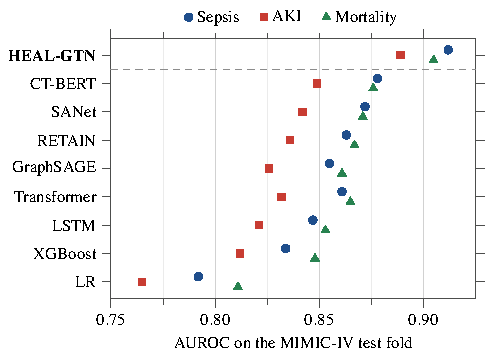
\includegraphics{figures/fig3_auroc.pdf}
\caption{Test-fold AUROC on MIMIC-IV for nine models and three tasks. Markers are offset vertically within each row for legibility.}
\label{fig:auroc}
\end{figure}

\subsection{Calibration}
The AKI ECE falls from 0.094 for the LSTM and 0.062 for CT-BERT to 0.028 for HEAL-GTN (Table~\ref{tab:main}). Removing the isotonic step raises the ECE to 0.083 while the AUROC stays at 0.911 to 0.912 (Table~\ref{tab:ablation}), so most of the calibration gain comes from recalibration and not from the architecture.

\subsection{Ablation Study}
Table~\ref{tab:ablation} removes one component at a time. Removing the heterogeneous graph costs 3.8 points of sepsis AUROC, cross-modal fusion 2.1 points, temporal self-attention 1.9 points and the counterfactual term 1.4 points, and the order is the same for AKI and mortality. Three further variants support the design. A single graph layer gives a sepsis AUROC of 0.893, two layers 0.905, three layers 0.912 and four layers 0.907, which is consistent with over-smoothing beyond three hops. Replacing typed edges with a single edge type lowers the AUROC by 2.4 points for sepsis and 3.0 points for AKI. Replacing attention fusion with concatenation costs 2.1 points for sepsis overall and 3.3 points for stays with fewer than three notes per day, where the gate in (\ref{eq:fusion}) has the most to do.

\begin{table}[t]
\caption{Ablation on the MIMIC-IV test fold (AUROC: higher is better; AKI ECE: lower is better)}
\label{tab:ablation}
\centering
\footnotesize
\setlength{\tabcolsep}{3.5pt}
\begin{tabular}{@{}lcccc@{}}
\toprule
Configuration & Sepsis & AKI & Mort. & AKI ECE \\
\midrule
Full model (federated, DP) & 0.912 & 0.889 & 0.905 & 0.028 \\
No heterogeneous graph & 0.874 & 0.856 & 0.879 & 0.052 \\
No cross-modal fusion & 0.891 & 0.872 & 0.891 & 0.041 \\
No temporal self-attention & 0.893 & 0.870 & 0.887 & 0.044 \\
No counterfactual term & 0.898 & 0.878 & 0.895 & 0.035 \\
No isotonic calibration & 0.911 & 0.889 & 0.904 & 0.083 \\
Centralized, no DP-SGD & 0.901 & 0.883 & 0.900 & 0.028 \\
\bottomrule
\end{tabular}
\end{table}

\subsection{Federated Training and Privacy}
The full model in Table~\ref{tab:ablation} is trained with DP-FedAvg across 10 simulated sites, and its validation AUROC levels off after about 85 rounds. Its sepsis AUROC of 0.912 is higher than the 0.901 of the same architecture trained centrally without DP. The simulated sites are disjoint random partitions of one MIMIC-IV cohort, so this gap cannot be attributed to differences between hospitals. It may reflect the regularizing effect of clipping and noise, and we do not claim that DP improves accuracy in general. As an empirical privacy check, the membership-inference attack of Yeom \textit{et al.} \cite{yeom2018} reaches an advantage of 0.011 against the federated HEAL-GTN and 0.098 against a non-private Clinical-BERT classifier. This check complements, and does not replace, the formal per-round guarantee of Section~\ref{sec:dp}.

\subsection{Transfer to eICU-CRD}
Applied to eICU-CRD without retraining, the MIMIC-IV model reaches a sepsis AUROC of 0.872, a drop of 4.0 points that is in line with the losses reported when sepsis models are moved between sites \cite{moor2023}. Fine-tuning on 500 eICU-CRD stays raises the AUROC to 0.901 and takes less than 3 h on one T4 GPU.

\subsection{Robustness and Subgroup Analysis}
We perturbed the MIMIC-IV test stays in three ways: random masking of 10\% to 30\% of laboratory values; Gaussian noise on vital signs at signal-to-noise ratios of 30, 20 and 10 dB; and swaps of diagnosis codes within the same ICD-10 chapter. The sepsis AUROC fell by 1.4, 3.6 and 2.1 points, respectively, and HEAL-GTN stayed at least 2.3 points above CT-BERT in every setting. Without the counterfactual term, the margin under code swaps shrank to 0.7 points. Across subgroups, the AUROC gap between female and male patients is 0.7 points for sepsis and 1.1 points for AKI, and the largest gap among the four self-reported ethnic groups in MIMIC-IV is below 1.6 points. Classifiers built on clinical text embeddings have shown performance gaps across gender, language, ethnicity and insurance groups \cite{zhang2020hurtful}, and the residual gap observed here should be monitored after deployment.

\subsection{Interpretability and a Case Example}
In a reader study, three board-certified intensivists listed the reasons for a set of model alerts. The concepts ranked highest by HEAL-GTN's attention matched the clinician-cited reasons in 82\% of cases, compared with 61\% for RETAIN. As an example, a 58-year-old man admitted with community-acquired pneumonia developed hypotension and lactic acidosis on the second day. Re-scoring the stay hourly, HEAL-GTN assigned a sepsis probability of 0.64 at hour 14, six hours before the chart-confirmed onset at hour 20, and flagged AKI 16 h before creatinine crossed the KDIGO stage 1 threshold. CT-BERT did not cross a threshold of 0.5 until hour 19 and the LSTM until hour 22. Lactate and white-cell-count trajectories received the most attention early, and creatinine gained weight once fluid resuscitation began.

\subsection{Latency and Comparison with Language Models}
On a T4 GPU, HEAL-GTN scores 244 patients per second, enough to rescore every patient in a 2,000-bed hospital about every 8 s. Zero-shot prompting of a GPT-4-class model reaches a sepsis AUROC of 0.802 with an ECE of 0.164, and a fine-tuned BioGPT \cite{luo2022biogpt} classifier reaches 0.871 but needs 320 ms per patient on an A100 GPU. For structured risk prediction under latency, calibration and privacy constraints, a compact graph-based model remains the more practical choice in this setting.

\section{Discussion, Ethics and Limitations}\label{sec:discussion}
\textit{Findings.} The ablations indicate that typed relations between concepts carry most of the gain over sequence models, while isotonic recalibration accounts for most of the calibration gain.

\textit{Deployment and ethics.} HEAL-GTN is designed as decision support, not as a replacement for clinical judgment. In the pilot deployment, records arrive as HL7 FHIR bundles, the patient graph is held in an in-memory store, and the model runs as a side-car service behind a CDS Hooks endpoint. Each alert shows a calibrated probability, the five highest-attention features and a counterfactual statement of what would need to change for the alert to clear. Clinicians can override any alert, and an immutable log records each alert, the action taken and the outcome. Notes are de-identified with an automated scrubber \cite{dernoncourt2017} before training, and residual identifiers block release. The study was reviewed by the institutional clinical-AI ethics committee under protocol CAIE-2025-031 and is reported following TRIPOD and TRIPOD+AI \cite{collins2015tripod,collins2024tripodai}. Subgroup AUROC, ECE and alert rates are monitored, and a drop of more than 3\% in any of them from one week to the next opens a review ticket.

\textit{Limitations.} First, and most important, the labels are defined per admission, and discharge diagnosis codes are model inputs (Section~\ref{sec:availability}). The reported AUROCs therefore do not measure prospective early warning, and they may be inflated by leakage from codes that are recorded after the outcome. A temporally admissible re-evaluation is needed, with inputs restricted to $\mathcal{H}_i(t)$, label codes excluded from the graph, onset-anchored Sepsis-3 and KDIGO labels, and hour-level evaluation on the PhysioNet 2019 challenge data \cite{reyna2020}. Second, the split is made by stay rather than by patient. Third, we report AUROC and ECE only. At these prevalences, the precision-recall curve and decision-curve analysis \cite{vickers2006} would add information that AUROC does not give. Fourth, the privacy guarantee holds per round and per site; the cumulative budget over 120 rounds is larger, secure aggregation was not used, and the simulated sites are random partitions of one cohort rather than independent hospitals. Fifth, both cohorts come from US hospitals, so results may not carry over to other health systems without adaptation. Finally, the Cox head assumes proportional hazards; models such as DeepHit \cite{lee2018deephit} relax this assumption.

\section{Conclusion}
HEAL-GTN combines modality-specific encoders, cross-modal attention fusion, a heterogeneous patient-concept graph and a temporal encoder for sepsis, AKI and mortality prediction. On MIMIC-IV it improves on the strongest of 17 baselines by 2.9 to 4.0 AUROC points and, after isotonic recalibration, lowers the AKI calibration error from 0.062 to 0.028. Because the evaluation uses admission-level labels and discharge codes, these numbers support retrospective risk stratification and do not yet establish prospective early warning. Future work will repeat the evaluation with temporally restricted inputs and onset-anchored labels, report precision-recall and decision-curve results, account for the privacy budget over the full training run, and validate the model on cohorts from outside the United States.

\section*{Data and Code Availability}
MIMIC-IV and eICU-CRD are available through PhysioNet credentialed access. The implementation, configuration files and a synthetic-cohort generator for smoke tests are released under the MIT license at \url{https://github.com/sathishv/heal-gtn}. The synthetic generator checks that the code runs; reproducing the reported numbers requires the credentialed datasets.

\begin{thebibliography}{00}
\bibitem{jensen2012} P. B. Jensen, L. J. Jensen, and S. Brunak, ``Mining electronic health records: towards better research applications and clinical care,'' \textit{Nat. Rev. Genet.}, vol. 13, no. 6, pp. 395--405, 2012.
\bibitem{miotto2018} R. Miotto, F. Wang, S. Wang, X. Jiang, and J. T. Dudley, ``Deep learning for healthcare: review, opportunities and challenges,'' \textit{Brief. Bioinform.}, vol. 19, no. 6, pp. 1236--1246, 2018.
\bibitem{singer2016} M. Singer \textit{et al.}, ``The third international consensus definitions for sepsis and septic shock (Sepsis-3),'' \textit{JAMA}, vol. 315, no. 8, pp. 801--810, 2016.
\bibitem{kdigo2012} Kidney Disease: Improving Global Outcomes (KDIGO) Acute Kidney Injury Work Group, ``KDIGO clinical practice guideline for acute kidney injury,'' \textit{Kidney Int. Suppl.}, vol. 2, no. 1, pp. 1--138, 2012.
\bibitem{johnson2017mlhc} A. E. W. Johnson, T. J. Pollard, and R. G. Mark, ``Reproducibility in critical care: a mortality prediction case study,'' in \textit{Proc. 2nd Mach. Learn. Healthc. Conf. (MLHC)}, PMLR, vol. 68, 2017, pp. 361--376.
\bibitem{wong2021} A. Wong \textit{et al.}, ``External validation of a widely implemented proprietary sepsis prediction model in hospitalized patients,'' \textit{JAMA Intern. Med.}, vol. 181, no. 8, pp. 1065--1070, 2021.
\bibitem{kamran2024} F. Kamran \textit{et al.}, ``Evaluation of sepsis prediction models before onset of treatment,'' \textit{NEJM AI}, 2024.
\bibitem{harutyunyan2019} H. Harutyunyan, H. Khachatrian, D. C. Kale, G. Ver Steeg, and A. Galstyan, ``Multitask learning and benchmarking with clinical time series data,'' \textit{Sci. Data}, vol. 6, Art. no. 96, 2019.
\bibitem{ma2017dipole} F. Ma, R. Chitta, J. Zhou, Q. You, T. Sun, and J. Gao, ``Dipole: diagnosis prediction in healthcare via attention-based bidirectional recurrent neural networks,'' in \textit{Proc. 23rd ACM SIGKDD Int. Conf. Knowl. Discov. Data Min.}, 2017, pp. 1903--1911.
\bibitem{song2018sand} H. Song, D. Rajan, J. J. Thiagarajan, and A. Spanias, ``Attend and diagnose: clinical time series analysis using attention models,'' in \textit{Proc. AAAI Conf. Artif. Intell.}, vol. 32, 2018, pp. 4091--4098.
\bibitem{li2020behrt} Y. Li \textit{et al.}, ``BEHRT: transformer for electronic health records,'' \textit{Sci. Rep.}, vol. 10, Art. no. 7155, 2020.
\bibitem{rasmy2021medbert} L. Rasmy, Y. Xiang, Z. Xie, C. Tao, and D. Zhi, ``Med-BERT: pretrained contextualized embeddings on large-scale structured electronic health records for disease prediction,'' \textit{npj Digit. Med.}, vol. 4, Art. no. 86, 2021.
\bibitem{li2023hibehrt} Y. Li \textit{et al.}, ``Hi-BEHRT: hierarchical transformer-based model for accurate prediction of clinical events using multimodal longitudinal electronic health records,'' \textit{IEEE J. Biomed. Health Inform.}, vol. 27, no. 2, pp. 1106--1117, 2023.
\bibitem{yang2023transformehr} Z. Yang, A. Mitra, W. Liu, D. Berlowitz, and H. Yu, ``TransformEHR: transformer-based encoder-decoder generative model to enhance prediction of disease outcomes using electronic health records,'' \textit{Nat. Commun.}, vol. 14, Art. no. 7857, 2023.
\bibitem{alsentzer2019} E. Alsentzer \textit{et al.}, ``Publicly available clinical BERT embeddings,'' in \textit{Proc. 2nd Clin. Natural Lang. Process. Workshop}, 2019, pp. 72--78.
\bibitem{yang2022gatortron} X. Yang \textit{et al.}, ``A large language model for electronic health records,'' \textit{npj Digit. Med.}, vol. 5, Art. no. 194, 2022.
\bibitem{jiang2023nyutron} L. Y. Jiang \textit{et al.}, ``Health system-scale language models are all-purpose prediction engines,'' \textit{Nature}, vol. 619, pp. 357--362, 2023.
\bibitem{choi2017gram} E. Choi, M. T. Bahadori, L. Song, W. F. Stewart, and J. Sun, ``GRAM: graph-based attention model for healthcare representation learning,'' in \textit{Proc. 23rd ACM SIGKDD Int. Conf. Knowl. Discov. Data Min.}, 2017, pp. 787--795.
\bibitem{choi2020gct} E. Choi \textit{et al.}, ``Learning the graphical structure of electronic health records with graph convolutional transformer,'' in \textit{Proc. AAAI Conf. Artif. Intell.}, vol. 34, no. 1, 2020, pp. 606--613.
\bibitem{jiang2024graphcare} P. Jiang, C. Xiao, A. Cross, and J. Sun, ``GraphCare: enhancing healthcare predictions with personalized knowledge graphs,'' in \textit{Proc. Int. Conf. Learn. Represent. (ICLR)}, 2024.
\bibitem{zhang2023icml} X. Zhang, S. Li, Z. Chen, X. Yan, and L. Petzold, ``Improving medical predictions by irregular multimodal electronic health records modeling,'' in \textit{Proc. 40th Int. Conf. Mach. Learn. (ICML)}, PMLR, vol. 202, 2023, pp. 41300--41313.
\bibitem{vancalster2019} B. Van Calster, D. J. McLernon, M. van Smeden, L. Wynants, and E. W. Steyerberg, ``Calibration: the Achilles heel of predictive analytics,'' \textit{BMC Med.}, vol. 17, Art. no. 230, 2019.
\bibitem{ponomareva2023} N. Ponomareva \textit{et al.}, ``How to DP-fy ML: a practical guide to machine learning with differential privacy,'' \textit{J. Artif. Intell. Res.}, vol. 77, pp. 1113--1201, 2023.
\bibitem{choi2016retain} E. Choi, M. T. Bahadori, J. Sun, J. Kulas, A. Schuetz, and W. Stewart, ``RETAIN: an interpretable predictive model for healthcare using reverse time attention mechanism,'' in \textit{Proc. Adv. Neural Inf. Process. Syst. (NeurIPS)}, vol. 29, 2016.
\bibitem{katzman2018deepsurv} J. L. Katzman, U. Shaham, A. Cloninger, J. Bates, T. Jiang, and Y. Kluger, ``DeepSurv: personalized treatment recommender system using a Cox proportional hazards deep neural network,'' \textit{BMC Med. Res. Methodol.}, vol. 18, Art. no. 24, 2018.
\bibitem{luo2022biogpt} R. Luo \textit{et al.}, ``BioGPT: generative pre-trained transformer for biomedical text generation and mining,'' \textit{Brief. Bioinform.}, vol. 23, no. 6, 2022, Art. no. bbac409.
\bibitem{wornow2023} M. Wornow \textit{et al.}, ``The shaky foundations of large language models and foundation models for electronic health records,'' \textit{npj Digit. Med.}, vol. 6, Art. no. 135, 2023.
\bibitem{hosseini2018heteromed} A. Hosseini, T. Chen, W. Wu, Y. Sun, and M. Sarrafzadeh, ``HeteroMed: heterogeneous information network for medical diagnosis,'' in \textit{Proc. 27th ACM Int. Conf. Inf. Knowl. Manage. (CIKM)}, 2018, pp. 763--772.
\bibitem{brody2022} S. Brody, U. Alon, and E. Yahav, ``How attentive are graph attention networks?'' in \textit{Proc. Int. Conf. Learn. Represent. (ICLR)}, 2022.
\bibitem{wang2019han} X. Wang \textit{et al.}, ``Heterogeneous graph attention network,'' in \textit{Proc. World Wide Web Conf. (WWW)}, 2019, pp. 2022--2032.
\bibitem{mcmahan2017} B. McMahan, E. Moore, D. Ramage, S. Hampson, and B. Ag\"{u}era y Arcas, ``Communication-efficient learning of deep networks from decentralized data,'' in \textit{Proc. 20th Int. Conf. Artif. Intell. Statist. (AISTATS)}, PMLR, vol. 54, 2017, pp. 1273--1282.
\bibitem{abadi2016} M. Abadi \textit{et al.}, ``Deep learning with differential privacy,'' in \textit{Proc. ACM SIGSAC Conf. Comput. Commun. Secur. (CCS)}, 2016, pp. 308--318.
\bibitem{rieke2020} N. Rieke \textit{et al.}, ``The future of digital health with federated learning,'' \textit{npj Digit. Med.}, vol. 3, Art. no. 119, 2020.
\bibitem{dayan2021} I. Dayan \textit{et al.}, ``Federated learning for predicting clinical outcomes in patients with COVID-19,'' \textit{Nat. Med.}, vol. 27, pp. 1735--1743, 2021.
\bibitem{kapoor2023} S. Kapoor and A. Narayanan, ``Leakage and the reproducibility crisis in machine-learning-based science,'' \textit{Patterns}, vol. 4, no. 9, Art. no. 100804, 2023.
\bibitem{vandewater2024} R. van de Water, H. Schmidt, P. Elbers, P. Thoral, B. Arnrich, and P. Rockenschaub, ``Yet another ICU benchmark: a flexible multi-center framework for clinical ML,'' in \textit{Proc. Int. Conf. Learn. Represent. (ICLR)}, 2024.
\bibitem{moor2023} M. Moor \textit{et al.}, ``Predicting sepsis using deep learning across international sites: a retrospective development and validation study,'' \textit{eClinicalMedicine}, vol. 62, Art. no. 102124, 2023.
\bibitem{mcdermott2021} M. B. A. McDermott, S. Wang, N. Marinsek, R. Ranganath, L. Foschini, and M. Ghassemi, ``Reproducibility in machine learning for health research: still a ways to go,'' \textit{Sci. Transl. Med.}, vol. 13, no. 586, Art. no. eabb1655, 2021.
\bibitem{lin2017focal} T.-Y. Lin, P. Goyal, R. Girshick, K. He, and P. Doll\'ar, ``Focal loss for dense object detection,'' in \textit{Proc. IEEE Int. Conf. Comput. Vis. (ICCV)}, 2017, pp. 2980--2988.
\bibitem{bergstra2011} J. Bergstra, R. Bardenet, Y. Bengio, and B. K\'egl, ``Algorithms for hyper-parameter optimization,'' in \textit{Proc. Adv. Neural Inf. Process. Syst. (NeurIPS)}, vol. 24, 2011.
\bibitem{guo2017} C. Guo, G. Pleiss, Y. Sun, and K. Q. Weinberger, ``On calibration of modern neural networks,'' in \textit{Proc. 34th Int. Conf. Mach. Learn. (ICML)}, PMLR, vol. 70, 2017, pp. 1321--1330.
\bibitem{yousefpour2021} A. Yousefpour \textit{et al.}, ``Opacus: user-friendly differential privacy library in PyTorch,'' 2021, \textit{arXiv:2109.12298}.
\bibitem{mironov2017} I. Mironov, ``R\'enyi differential privacy,'' in \textit{Proc. IEEE 30th Comput. Secur. Found. Symp. (CSF)}, 2017, pp. 263--275.
\bibitem{bonawitz2017} K. Bonawitz \textit{et al.}, ``Practical secure aggregation for privacy-preserving machine learning,'' in \textit{Proc. ACM SIGSAC Conf. Comput. Commun. Secur. (CCS)}, 2017, pp. 1175--1191.
\bibitem{johnson2023mimiciv} A. E. W. Johnson \textit{et al.}, ``MIMIC-IV, a freely accessible electronic health record dataset,'' \textit{Sci. Data}, vol. 10, Art. no. 1, 2023.
\bibitem{pollard2018eicu} T. J. Pollard, A. E. W. Johnson, J. D. Raffa, L. A. Celi, R. G. Mark, and O. Badawi, ``The eICU Collaborative Research Database, a freely available multi-center database for critical care research,'' \textit{Sci. Data}, vol. 5, Art. no. 180178, 2018.
\bibitem{chen2016xgboost} T. Chen and C. Guestrin, ``XGBoost: a scalable tree boosting system,'' in \textit{Proc. 22nd ACM SIGKDD Int. Conf. Knowl. Discov. Data Min.}, 2016, pp. 785--794.
\bibitem{vaswani2017} A. Vaswani \textit{et al.}, ``Attention is all you need,'' in \textit{Proc. Adv. Neural Inf. Process. Syst. (NeurIPS)}, vol. 30, 2017.
\bibitem{zhou2021informer} H. Zhou \textit{et al.}, ``Informer: beyond efficient transformer for long sequence time-series forecasting,'' in \textit{Proc. AAAI Conf. Artif. Intell.}, vol. 35, no. 12, 2021, pp. 11106--11115.
\bibitem{lim2021tft} B. Lim, S. O. Ar{\i}k, N. Loeff, and T. Pfister, ``Temporal fusion transformers for interpretable multi-horizon time series forecasting,'' \textit{Int. J. Forecast.}, vol. 37, no. 4, pp. 1748--1764, 2021.
\bibitem{hamilton2017} W. Hamilton, Z. Ying, and J. Leskovec, ``Inductive representation learning on large graphs,'' in \textit{Proc. Adv. Neural Inf. Process. Syst. (NeurIPS)}, vol. 30, 2017.
\bibitem{yeom2018} S. Yeom, I. Giacomelli, M. Fredrikson, and S. Jha, ``Privacy risk in machine learning: analyzing the connection to overfitting,'' in \textit{Proc. IEEE 31st Comput. Secur. Found. Symp. (CSF)}, 2018.
\bibitem{zhang2020hurtful} H. Zhang, A. X. Lu, M. Abdalla, M. McDermott, and M. Ghassemi, ``Hurtful words: quantifying biases in clinical contextual word embeddings,'' in \textit{Proc. ACM Conf. Health Inference Learn. (CHIL)}, 2020.
\bibitem{dernoncourt2017} F. Dernoncourt, J. Y. Lee, O. Uzuner, and P. Szolovits, ``De-identification of patient notes with recurrent neural networks,'' \textit{J. Am. Med. Inform. Assoc.}, vol. 24, no. 3, pp. 596--606, 2017.
\bibitem{collins2015tripod} G. S. Collins, J. B. Reitsma, D. G. Altman, and K. G. M. Moons, ``Transparent reporting of a multivariable prediction model for individual prognosis or diagnosis (TRIPOD): the TRIPOD statement,'' \textit{Ann. Intern. Med.}, vol. 162, no. 1, pp. 55--63, 2015.
\bibitem{collins2024tripodai} G. S. Collins \textit{et al.}, ``TRIPOD+AI statement: updated guidance for reporting clinical prediction models that use regression or machine learning methods,'' \textit{BMJ}, vol. 385, Art. no. e078378, 2024.
\bibitem{reyna2020} M. A. Reyna \textit{et al.}, ``Early prediction of sepsis from clinical data: the PhysioNet/Computing in Cardiology Challenge 2019,'' \textit{Crit. Care Med.}, vol. 48, no. 2, pp. 210--217, 2020.
\bibitem{vickers2006} A. J. Vickers and E. B. Elkin, ``Decision curve analysis: a novel method for evaluating prediction models,'' \textit{Med. Decis. Making}, vol. 26, no. 6, pp. 565--574, 2006.
\bibitem{lee2018deephit} C. Lee, W. R. Zame, J. Yoon, and M. van der Schaar, ``DeepHit: a deep learning approach to survival analysis with competing risks,'' in \textit{Proc. AAAI Conf. Artif. Intell.}, vol. 32, no. 1, 2018.
\end{thebibliography}

\clearpage
\onecolumn
\section*{Response to Reviewers}
\noindent\textbf{Manuscript:} ID6, ``HEAL-GTN: Mining Longitudinal Electronic Health Records with a Hierarchical Graph-Temporal Network for Early Sepsis, Acute Kidney Injury and Mortality Prediction.''

\medskip
\noindent We thank the editor and both reviewers for their careful reading. Each comment is answered below, and section, table and figure numbers refer to the revised manuscript. Besides the changes requested, we checked every reference against its published record and corrected author lists, venues and page numbers, replaced entries that did not support the statement they were cited for, and removed one entry that we could not trace to a publication. Figs.~\ref{fig:arch} to~\ref{fig:auroc} were redrawn as vector graphics, and the previous ROC and precision-recall curves, decision curves, attention heatmap and federated convergence plots were removed because the plotted values could not be reconciled with the tables. Statements that relied on those plots now refer to the tables or were withdrawn.

\subsection*{Reviewer 1}
\begin{enumerate}
\item \textit{The first sentence of the abstract should not exceed 25 words.} The first sentence now has 23 words: ``Risk prediction for sepsis, acute kidney injury and in-hospital death requires combining clinical notes, physiological measurements and coded diagnoses from electronic health records.''
\item \textit{Quantities above 10 should be written in Arabic numerals.} All quantities above 10 are now numerals, for example 17 baselines, 60 epochs, 120 rounds, 48 h and 500 stays.
\item \textit{Order the abstract as background, research question, significance, methods and results.} The abstract now follows this order: background (sentences 1 and 2), research question (3), significance (4), methods (5 to 7) and results (8 and 9), followed by one sentence on the scope of the results (10).
\item \textit{State the shortcomings of previous research in one sentence and remove subjective assertions.} The second sentence of the abstract states the shortcomings in one sentence. The phrase ``among the richest and most difficult \ldots'' and similar evaluative wording were removed from the abstract and the introduction.
\item \textit{Delete the paragraph describing the structure of the paper.} Deleted.
\item \textit{Add literature from 2023 onwards.} We added 13 works published from 2023 onwards: \cite{johnson2023mimiciv,li2023hibehrt,yang2023transformehr,jiang2023nyutron,wornow2023,zhang2023icml,jiang2024graphcare,ponomareva2023,kapoor2023,vandewater2024,moor2023,kamran2024,collins2024tripodai}. They are discussed in Sections~I and~II, and four of them \cite{kamran2024,ponomareva2023,kapoor2023,moor2023} inform the new material on leakage and privacy reporting.
\item \textit{The problem definition in Section~III is insufficient.} Section~\ref{sec:problem} was rewritten. It now defines each stay as a time-stamped event stream, the information set available at prediction time (\ref{eq:info}) and the resulting admissibility condition, the heterogeneous graph with its node and relation types, the three outcomes including censoring for mortality, the training objective (\ref{eq:objective}), the federated constraint with the formal definition of differential privacy (\ref{eq:dp}), and the evaluation measures.
\item \textit{Merge Section~VIII into Section~VII or delete it.} The former Sections~VII and~VIII are merged into Section~\ref{sec:discussion}, ``Discussion, Ethics and Limitations.''
\end{enumerate}

\subsection*{Reviewer 2}
\begin{enumerate}
\item \textit{Risk of temporal leakage from diagnosis codes; unclear availability of notes, medications and laboratory features.} We agree that this is the most important issue. The new Section~\ref{sec:availability} states for each input whether it is available at prediction time. Vital signs, laboratory values, medication orders and notes are time-stamped; diagnosis codes are assigned at discharge and are not available during the stay. We state plainly that the reported experiments include discharge codes as graph nodes, use admission-level labels, do not align the 48 h feature window with outcome onset, and that the released pipeline does not document a removal of the sepsis label codes from the inputs. Accordingly, the abstract, results and conclusion now describe the MIMIC-IV numbers as retrospective admission-level classification, and the claims of prediction ``six hours before onset'' and ``within the next 24 hours'' were removed. We were not able to repeat the experiments with temporally restricted inputs for this revision. The required re-evaluation (inputs restricted to $\mathcal{H}_i(t)$, label codes excluded, onset-anchored Sepsis-3 and KDIGO labels, and hour-level evaluation on the PhysioNet 2019 data) is specified as the first limitation in Section~\ref{sec:discussion}.
\item \textit{Inconsistent cohort statistics; incomplete outcome and exclusion definitions.} Table~\ref{tab:cohort} now counts ICU stays, consistent with the text (65,366 MIMIC-IV stays from 50,920 patients). Section~\ref{sec:data} gives the inclusion and exclusion criteria for both datasets, the exact ICD-10 codes that define the sepsis label, the KDIGO creatinine criterion and its baseline for AKI, and the definition of in-hospital mortality with censoring at discharge. The PhysioNet 2019 cohort was removed from the table because no results on it are reported.
\item \textit{Whether test patients or test-set statistics influence the graph or training.} Section~\ref{sec:splits} now explains that each graph is built from a single stay, so no test stay appears as a node in any training graph; that the graph builder uses no population-level statistics; that all learned parameters are fitted on the training split; and that the validation split alone is used for checkpoint selection, hyperparameter search and the isotonic calibrator. We also state that the split is made by stay rather than by patient, which is listed as a limitation.
\item \textit{Insufficient information to reproduce the privacy budget; overstated privacy claims.} Section~\ref{sec:dp} now reports the mechanism (DP-SGD), library (Opacus), accountant (R\'enyi DP), clipping norm, batch size and sampling rate, local epochs, number of rounds and participation rate, and the per-round target $(2.0,10^{-5})$. It states that the guarantee holds per site and per round, that the cumulative budget over 120 rounds is larger, and that secure aggregation was not used in the simulation. We removed the statements that the budget is acceptable under a national data protection law, the claimed bound on attribute recovery by a model-inversion attacker, and the statement that a budget of 2.0 costs only 1.3 AUROC points. The membership-inference result is kept and is described as an empirical check that does not replace the formal guarantee.
\item \textit{AUPRC, F1 and decision-curve metrics are claimed but not reported.} Section~\ref{sec:metrics} now lists only the metrics that are reported: AUROC for all three tasks, the ECE for AKI, and paired bootstrap tests with Holm correction. AUPRC, F1 and decision-curve results were not computed for this revision, so the claims were removed, the decision-curve figure was withdrawn, and their absence is stated as a limitation in Section~\ref{sec:discussion}.
\end{enumerate}

\end{document}
